%----------------------------------------------------------------------------
\chapter{\projectlifecycle}
%----------------------------------------------------------------------------

A projektmenedzsment egyik alapvető elve, hogy minden projekt rendelkezik egy jól definiált életciklussal, 
amely több, egymásra épülő fázisra bontható. 
Ez az életciklus nemcsak logikai és időbeli folyamatot ír le, hanem szervezeti, irányítási és ellenőrzési szempontból is meghatározó, 
hiszen lehetővé teszi a projekt strukturált tervezését, a folyamatok nyomon követését, a kockázatok kezelését és a teljesítmény értékelését \cite{Szalay2018,Hajdu2014,Kaposi2019}. 

A hazai szakirodalom rendszerint öt alapvető fázist különít el \cite{Kovacs2016,Simon2015}:

\begin{enumerate}
    \item \textbf{Projektindítás (Initiation):} a projekt céljainak, indokoltságának, és a legfontosabb paraméterek meghatározása.
    \item \textbf{Tervezés (Planning):} részletes ütemezés, erőforrás-tervezés, kockázatelemzés és feladatdefiniálás.
    \item \textbf{Megvalósítás (Execution):} a projekt tényleges kivitelezése, fejlesztés és implementáció.
    \item \textbf{Ellenőrzés és irányítás (Monitoring \& Controlling):} az előrehaladás, a költségek, az idő és a minőség folyamatos nyomon követése.
    \item \textbf{Lezárás (Closure):} a projekt hivatalos befejezése, átadás, visszacsatolás és a tapasztalatok dokumentálása.
\end{enumerate}

%----------------------------------------------------------------------------
\begin{figure}[H]
    \centering
    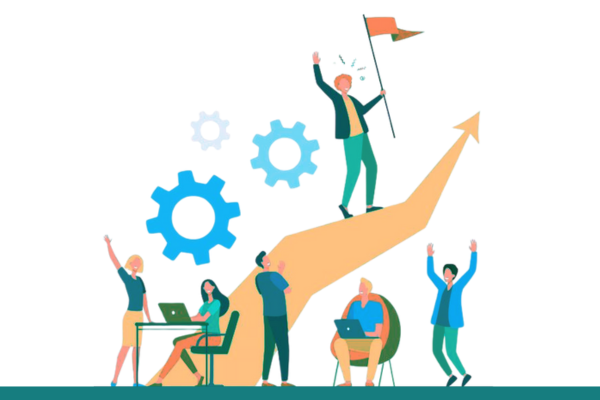
\includegraphics[width=50mm, keepaspectratio]{figures/project_creative.png}
    \caption{Projekt kreatív vizualizáció}
    \label{fig:project_creative}
\end{figure}
%----------------------------------------------------------------------------

A fázisok egymásra épülnek, de gyakran átfedésben is zajlanak: például az ellenőrzési és irányítási tevékenység a megvalósítás teljes időtartama alatt folyamatosan jelen van. 
A modern, iteratív fejlesztési modellek — mint az Agile vagy Scrum — nem feltétlenül követik a klasszikus lineáris struktúrát, 
hanem sprint-alapú, ciklikus megközelítést alkalmaznak \cite{Hajdu2014,Kaposi2019}.

A klasszikus ötfázisú modell azonban stratégiai és vállalati projekteknél továbbra is nélkülözhetetlen, 
mivel átlátható keretet biztosít a projekt teljes életciklusára. 
A \textbf{TeDeRMS} fejlesztése során is ez a modell szolgált alapul, amelyet a projekt sajátosságaihoz — önálló fejlesztés, korlátozott erőforrások és vállalati integráció — igazítottam.

%----------------------------------------------------------------------------
\section{Projektindítás (Initiation)}
%----------------------------------------------------------------------------

A projektindítás szakasza a projekt életciklusának alapvető lépése, mivel meghatározza a projekt céljait, irányait és kereteit. 
A kezdeti fázis során végzett tevékenységek minősége közvetlen hatással van a projekt kockázatkezelésére, a mérföldkövek elérésére és a költséghatékonyságra. 
A projekt sikeressége nagymértékben függ a kezdeti igényfeltárás alapos elvégzésétől \cite{Hajdu2014,Szalay2018,Kovacs2016,Kaposi2019}.

%----------------------------------------------------------------------------
\subsection{Igényfelmérés}
%----------------------------------------------------------------------------

A vállalat bérléskezelési folyamatait részletesen feltérképeztem.
Az igényfelmérés célja a folyamatok és a problémás területek feltárása, amely biztosítja a projekt következő szakaszainak sikeres végrehajtását, 
ez segít a kockázatok korai azonosítását a funkciók valós vállalati igényekhez való illesztését.  
Emellett fontos a szervezeti kontextus és az érintettek szempontjainak figyelembevétele, mivel ez növeli a projekt elfogadottságát és annak végrehajtásának hatékonyságát \cite{Kovacs2016,Kaposi2019}.

%----------------------------------------------------------------------------
\subsection{Célok meghatározása}
%----------------------------------------------------------------------------

Világos, mérhető célokat tűztem ki, például az adminisztrációs idő lecsökkentését, az adatpontosság javítását és az automatizált riportok bevezetését.  
A célok meghatározása biztosítja a projekt fókuszát és elősegíti az erőforrások optimális elosztását, valamint biztosítják a teljesítmény objektív értékelését.
A hierarchikus rendszere támogatja a stratégiai, taktikai és operatív döntések összehangolását, valamint a projektmenedzsment folyamatok átláthatóságát \cite{Hajdu2014,Szalay2018}.

%----------------------------------------------------------------------------
\subsection{Erőforrás-tervezés előkészítése}
%----------------------------------------------------------------------------

A projekt kezdetén meghatároztam a fejlesztés technológiai és időbeli erőforrásigényét.  
Mivel a munkát önállóan végeztem, kiemelten fontos volt a prioritások pontos kijelölése és a munkaidő hatékony beosztása.  
Az erőforrás-tervezés előkészítése hozzájárult a rendelkezésre álló kapacitások optimális elosztásához, 
a munkafolyamatok hatékony megszervezéséhez, valamint a feladatok közötti egyensúly megőrzéséhez. 

A részletes erőforrás-tervezés segíti a rugalmasság megőrzését, a váratlan események gyors kezelését,  
és a mérföldkövek teljesítését a tervezett idő- és költségkereten belül \cite{Kovacs2016,Kaposi2019,Hajdu2014}.  

%----------------------------------------------------------------------------
\section{Tervezés (Planning)}
%----------------------------------------------------------------------------

A tervezés szakasza kritikus jelentőségű a projekt sikerének biztosításában, mivel ekkor kerülnek meghatározásra az ütemezés, az erőforrások elosztása és a kockázatok kezelése. 
A részletes és előrelátó tervezés segítette minimalizálni a váratlan problémák hatását, előre jelezve a potenciális kockázatokat, 
és ez támogatta a projekt teljesítményének nyomon követését \cite{Hajdu2014,Szalay2018,Kovacs2016,Kaposi2019}.

%----------------------------------------------------------------------------
\subsection{Ütemterv készítése}
%----------------------------------------------------------------------------

A projekt kezdeti szakaszában elkészítettem a részletes ütemtervet, amely a fő mérföldköveket és a feladatokat logikai és időbeli sorrendbe rendezte.  
Ez a folyamat biztosította a fejlesztés előrehaladásának nyomon követését, valamint a feladatok közötti függőségek pontos feltérképezését.  

A jól felépített ütemterv hozzájárult az adott feladat teljesítéséhez és ellenőrzéséhez, emellett segített az erőforrások hatékony elosztásában \cite{Kovacs2016,Kaposi2019}.  
A projekt előrehaladásának dokumentálását is támogatta,  
ami elengedhetetlen a projektmenedzsment ellenőrzési és értékelési folyamataihoz.

%----------------------------------------------------------------------------
\subsection{Erőforrás-tervezés}
%----------------------------------------------------------------------------

Az erőforrás-tervezés során a rendelkezésre álló humán és technológiai kapacitások felmérése és optimális elosztása kulcsfontosságú volt.  
A részletes erőforrás-tervezés előmozdította a projekt rugalmasságát, elősegítette a prioritások helyes meghatározását, és csökkentette a késedelmek kockázatát \cite{Hajdu2014,Szalay2018}.  
Saját tapasztalatom alapján különösen kiscsapatos vagy önálló fejlesztési környezetben a munkaidő hatékony beosztása, valamint a terhelés és pihenőidő egyensúlya alapvető fontosságú.  
Ez a szemlélet nemcsak a projekt előrehaladását, hanem a minőségi kivitelezést is jelentősen támogatja.

%----------------------------------------------------------------------------
\begin{figure}[H]
    \centering
    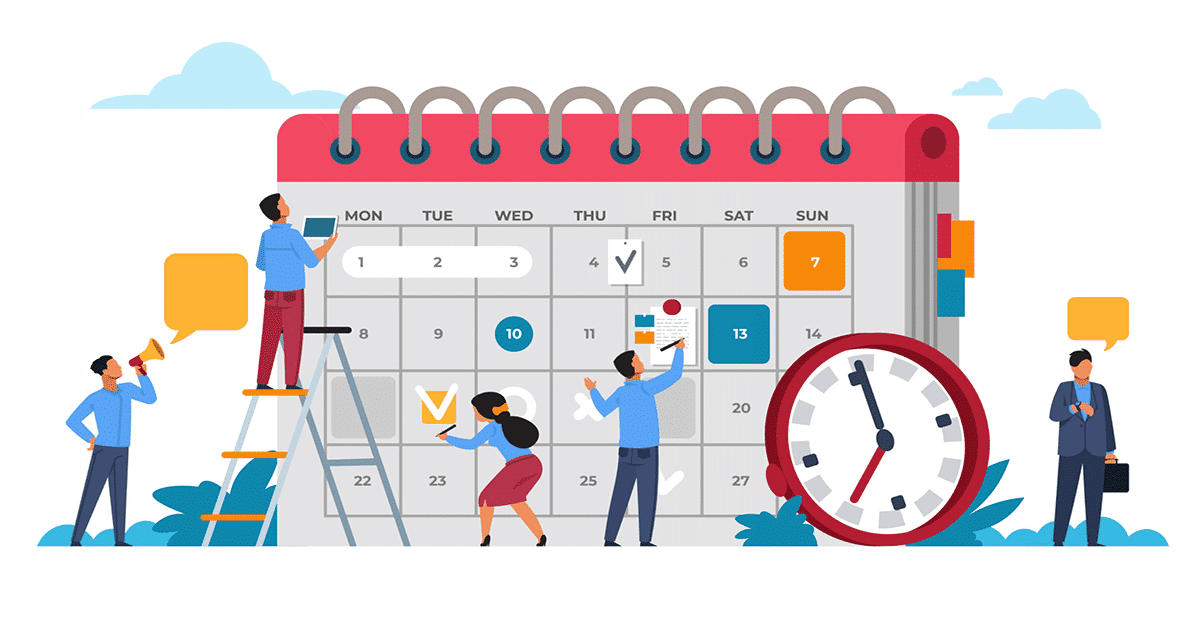
\includegraphics[width=70mm, keepaspectratio]{figures/plan.png}
    \caption{Naptári ütemterv vizualizáció}
    \label{fig:plan}
\end{figure}
%----------------------------------------------------------------------------

%----------------------------------------------------------------------------
\subsection{Kockázatelemzés}
%----------------------------------------------------------------------------

A projekt tervezési szakaszában részletes kockázatelemzést végeztem, amelynek során azonosítottam a főbb veszélyforrásokat — többek között a technikai hibákat, 
az esetleges adatvesztést és az üzleti logika működésében rejlő kockázatokat.  
Ezekre kidolgoztam mind megelőző, mind elhárító intézkedéseket, amelyek célja a problémák előfordulásának minimalizálása, illetve a gyors kezelése volt.  

A kockázatelemzés során alkalmazott kockázatmátrix megkönnyítette a lehetséges események valószínűségének és hatásának objektív értékelését, 
ezáltal támogatva a priorizálást és a döntéshozatalt \cite{Kovacs2016,Kaposi2019}.  
Ez a módszertan nagymértékben hozzájárult a projekt stabilitásához és a váratlan események hatékony kezeléséhez.  

Tehát a kockázatelemzés nem csupán egy formális projektmenedzsment-eszköz, hanem egy gondolkodásmód is, 
amely segít előre látni a problémákat és felkészülni rájuk \cite{Hajdu2014,Szalay2018}.

%----------------------------------------------------------------------------
\section{Megvalósítás (Execution)}
%----------------------------------------------------------------------------

A megvalósítás szakasza a projekt tényleges kivitelezését foglalja magában, amely során a tervezett funkciók, 
folyamatok és erőforrások gyakorlati alkalmazásra kerülnek. Ebben a fázisban a projektmenedzsment 
és a technikai végrehajtás szoros összhangja kulcsfontosságú a kívánt eredmények eléréséhez \cite{Hajdu2014,Szalay2018,Kaposi2019}.

%----------------------------------------------------------------------------
\subsection{Fejlesztési folyamatok}
%----------------------------------------------------------------------------

A fejlesztési folyamatok során kiemelt szerepet kapott a moduláris architektúra kialakítása, amely megalapozta a rendszer különálló komponenseinek önálló fejlesztését és tesztelését.  
Ez a megközelítés nemcsak a párhuzamos munkavégzést tette lehetővé, hanem a hibák gyorsabb azonosítását és javítását is segítette, így növelve a fejlesztés hatékonyságát és stabilitását.  

A moduláris szerkezet mellett a verziókövető rendszer, konkrétan a GitHub, alapvető eszközként szolgált a fejlesztés átláthatóságának 
fenntartásához és a kód integritásának megőrzéséhez.  
A verziókezelés segítségével minden módosítás pontosan visszakövethetővé vált, ami különösen fontos volt az önálló fejlesztés során, 
hiszen így a hibák eredete gyorsan beazonosítható volt \cite{Kovacs2016,Kaposi2019}.  

A backend és frontend komponensek párhuzamos fejlesztése szintén elősegítette az erőforrások hatékonyabb kihasználását.  
Ez a munkaszervezési stratégia nemcsak időmegtakarítást eredményezett, hanem lehetőséget teremtett a különböző funkcionális modulok 
egyidejű tesztelésére is, így a projekt előrehaladása folyamatos és jól kontrollált maradt.

%----------------------------------------------------------------------------
\subsection{Tesztelés}
%----------------------------------------------------------------------------

A tesztelés a megvalósítási fázis egyik legkritikusabb eleme, mivel közvetlenül befolyásolja a rendszer stabilitását, megbízhatóságát és a hosszú távú fenntarthatóságát.  
A folyamatos és módszeres tesztelés segítette a hibák korai felismerését, ezáltal csökkentve azok későbbi előfordulásának kockázatát.  
A rendszeres ellenőrzési ciklusok hozzájárultak ahhoz, hogy a fejlesztés iteratív módon, kontrolláltan és minőségbiztosítási szempontból is megalapozottan haladjon előre.  

A tesztelési folyamat két fő szintre tagolódott: egyrészt az \textit{unit tesztek} az egyes modulok működését ellenőrizték, 
biztosítva, hogy minden komponens önállóan is megfelelően funkcionáljon,  
másrészt a \textit{funkcionális tesztek} a rendszer egészének integrált működését vizsgálták, különös tekintettel az üzleti 
logika helyességére és a felhasználói élmény konzisztenciájára \cite{Szalay2018,Hajdu2014}.  

A folyamatos validálási szemlélet nemcsak a hibák számát csökkentette, hanem hozzájárult a fejlesztés átláthatóságához és a minőség folyamatos fenntartásához is,  
ezáltal megalapozva a rendszer hosszú távú megbízhatóságát és üzemeltetési biztonságát.

%----------------------------------------------------------------------------
\subsection{Dokumentáció}
%----------------------------------------------------------------------------

A dokumentáció a projekt hosszú távú fenntarthatóságának és minőségbiztosításának alapvető pillére.  
A fejlesztés során készített részletes kód- és rendszerleírás nem csupán a karbantartás és a jövőbeli bővítések megkönnyítését szolgálta,  
hanem a fejlesztési folyamatok átláthatóságát és a visszakövethetőségét is biztosította.  

A dokumentáció elkészítése során különös figyelmet fordítottam a logikai felépítésre, a modulok közötti összefüggésekre és az alkalmazott technológiák 
részletes ismertetésére, így a rendszer működése és szerkezete bármikor visszakövethetővé vált. 
Ez különösen fontos volt az önálló fejlesztés szempontjából, hiszen a dokumentálás nemcsak a saját munkám későbbi értelmezését segítette,  
hanem megteremtette a lehetőséget a projekt más fejlesztők általi folytatására is \cite{Kovacs2016,Kaposi2019,Szalay2018}.  

A megvalósítási szakasz így nemcsak a szoftver működési stabilitását, hanem a projekt átláthatóságát és minőségét is megalapozta,  
biztosítva, hogy a rendszer minden funkciója a terveknek megfelelően valósuljon meg, és hosszú távon is hatékonyan szolgálja a vállalat igényeit \cite{Hajdu2014}.

%----------------------------------------------------------------------------
\section{Ellenőrzés és irányítás (Monitoring és Controlling)}
%----------------------------------------------------------------------------

Az ellenőrzés és irányítás fázisa a projekt sikerének egyik legfontosabb garanciája, mivel biztosítja, 
hogy a tervezett célok teljesüljenek, az erőforrások optimálisan legyenek felhasználva, 
és a projekt kockázatai időben kezelhetők legyenek \cite{Hajdu2014,Szalay2018,Kovacs2016,Kaposi2019}. 
A monitoring és controlling nem csupán a problémák felderítésére szolgál, 
hanem a proaktív beavatkozást és a projekt folyamatos finomhangolását is.

%----------------------------------------------------------------------------
\subsection{Haladás nyomon követése}
%----------------------------------------------------------------------------

A projekt sikeres megvalósítása érdekében a haladás folyamatos nyomon követése alapvetően szükséges.  
A mérföldkövek rendszeres nyomon követése segít a projekt ütemtervének betartásában, és időben feltárja az esetleges eltéréseket.

A folyamatos monitorozás segít a késedelmek és az erőforrás-túlhasználat megelőzésében,  
valamint támogatja a szükséges korrekciók gyors és célzott végrehajtását.  
Ez a megközelítés javítja a projekt átláthatóságát és erősíti a vezetői döntések megalapozottságát,  
hiszen az objektív teljesítménymutatók alapján lehet meghatározni a szükséges beavatkozásokat \cite{Kovacs2016,Kaposi2019}.  

%----------------------------------------------------------------------------
\subsection{Kockázatok kezelése}
%----------------------------------------------------------------------------

A potenciális problémák hatásának minimalizálása érdekében elengedhetetlen, hogy a kockázatokat folyamatosan azonosítsuk, értékeljük és azokat nyomon kövessük.  

A kockázatmátrix folyamatos frissítése által, az új kockázatok időbeni azonosítása, 
a valószínűség és a hatás pontos értékelése, valamint a megfelelő megelőző intézkedések és vészforgatókönyvek kidolgozása könnyebbé válik.
Ez a preventív megközelítés nemcsak a váratlan események negatív következményeit csökkenti,  
hanem hozzájárul a projekt idő- és költségkeretének betartásához, és növeli a fejlesztés egészének sikerességét \cite{Hajdu2014,Szalay2018}.  

A kockázatkezelés ezen módja adja a döntéshozatal megalapozottságát,  
és biztosítja, hogy a projekt minden fázisában a problémák hatékonyan, gyorsan és kontrolláltan legyenek kezelve.

%----------------------------------------------------------------------------
\begin{figure}[H]
    \centering
    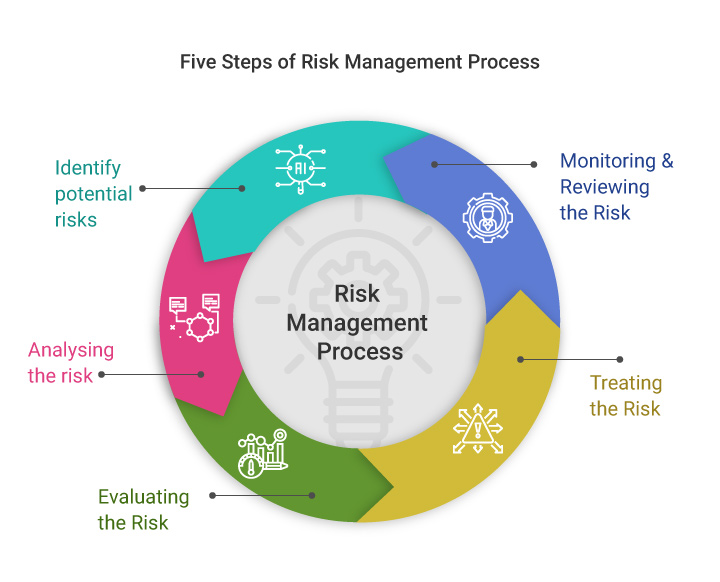
\includegraphics[width=70mm, keepaspectratio]{figures/risk.jpg}
    \caption{Kockázatkezelés példa}
    \label{fig:risk}
\end{figure}
%----------------------------------------------------------------------------

%----------------------------------------------------------------------------
\subsection{Minőségellenőrzés}
%----------------------------------------------------------------------------

A minőségellenőrzés célja, hogy a rendszer minden funkciója megfeleljen a tervezett követelményeknek, 
és a hibák a lehető legkorábban azonosításra kerüljenek.
A folyamatos ellenőrzés elősegíti a rendszer stabilitását és megbízhatóságát, támogatja az iteratív 
javítási folyamatokat, és hozzájárul a projekt sikeres lezárásához \cite{Kovacs2016,Kaposi2019,Szalay2018}.
Emellett az irányítási és monitoring tevékenységek biztosítják, hogy a mérföldkövek teljesüljenek, 
a minőségi elvárások teljesüljenek, valamint lehetőséget adnak a folyamatok optimalizálására.

%----------------------------------------------------------------------------
\section{Projekt lezárás (Closure)}
%----------------------------------------------------------------------------

A projekt lezárása a projektmenedzsment egyik kritikus fázisa, amikor a fejlesztett rendszer átadásra kerül, 
és a projekt során szerzett tapasztalatok összegzésre kerülnek.  
Ez a szakasz biztosítja a rendszer hosszú távú fenntarthatóságát, a felhasználói igények teljesítését, valamint 
a projekt teljesítményének és minőségének dokumentált értékelését \cite{Hajdu2014,Szalay2018,Kovacs2016,Kaposi2019}.

%----------------------------------------------------------------------------
\subsection{Rendszer átadása}
%----------------------------------------------------------------------------

A \textbf{TeDeRMS} telepítése a vállalat környezetében során a rendszer funkcionalitásának és stabilitásának biztosítása az elsődleges cél.  
Fontos, hogy az átadás során a rendszer zökkenőmentesen üzemeljen, és a felhasználók számára azonnal használható legyen.  

Az átadás során a folyamatok zavartalan működését elősegítő intézkedések, például a telepítési ellenőrzőlisták és 
a felhasználói oktatás, jelentősen csökkentik a támogatási igényt és növelik a rendszer elfogadottságát.  
Ez a lépés így nem csupán technikai feladat, hanem kulcsfontosságú a projekt sikeres lezárása és a vállalat napi működésének támogatása szempontjából.


%----------------------------------------------------------------------------
\subsection{Felhasználói és adminisztrátori dokumentáció}
%----------------------------------------------------------------------------

A projekt lezárásának fontos része a részletes dokumentáció elkészítése, amely felhasználói és adminisztrátori kézikönyveket foglal magában.  
Ez lehetővé teszi, hogy a rendszer működését, konfigurációját és funkcióit később bárki könnyen megértse és kezelje.  

A dokumentáció nem csupán útmutató a felhasználók számára, hanem támogatja a karbantartást, a jövőbeli bővítéseket, valamint biztosítja az auditálás és a minőségellenőrzés alapját.  
A jól strukturált, részletes dokumentáció így közvetlenül megerősíti a rendszer hosszú távú fenntarthatóságához és a projekt eredményességéhez \cite{Hajdu2014,Kaposi2019}.


%----------------------------------------------------------------------------
\subsection{Oktatás és képzés}
%----------------------------------------------------------------------------

A projekt lezárásának kulcsfontosságú része a felhasználók képzése, amely során a kulcsfelhasználók megismerkednek a rendszer működésével és funkcióival.  
A megfelelő oktatás biztosítja, hogy a rendszer a vállalatnál maximális hatékonysággal legyen alkalmazható, és növeli a felhasználói elfogadottságot.  

A képzés közvetlenül segít a hibák csökkentéséhez és a napi működés zavartalanságához, mivel a felhasználók magabiztosan tudják kezelni a rendszert.  
Emellett az oktatás révén a vállalat csökkentheti a belső támogatási igényeket, és a rendszer önálló, hatékony használatát \cite{Szalay2018,Kovacs2016}.

\begin{comment}
%----------------------------------------------------------------------------
\subsection{Tanulságok összegzése}
%----------------------------------------------------------------------------

A projekt lezárásának kulcsfontosságú eleme a tanulságok összegzése, amely elősegíti 
a szervezeti tudás megőrzését és a folyamatok folyamatos fejlesztését.
A projekt során szerzett tapasztalatok dokumentálása segíti a jövőbeli projektek 
tervezését, a hibák elkerülését, és támogatja a hatékonyabb projektmenedzsment kialakítását.  

A tapasztalatok rögzítése hozzájárul a vállalati projektek hosszú távú sikerességéhez és stabilitásához.  
Emellett a tanulságok összegzése lehetőséget ad a meglévő folyamatok finomhangolására, az erőforrások jobb elosztására, 
és a stratégiai döntéshozatal megalapozására \cite{Hajdu2014,Szalay2018,Kaposi2019}.  
Ez a szakasz biztosítja, hogy a rendszer fenntarthatóan, hatékonyan működjön, miközben 
a projektmenedzsment tapasztalatai a későbbiekben is hasznosíthatók maradnak.
\end{comment}

%----------------------------------------------------------------------------
\begin{figure}[H]
    \centering
    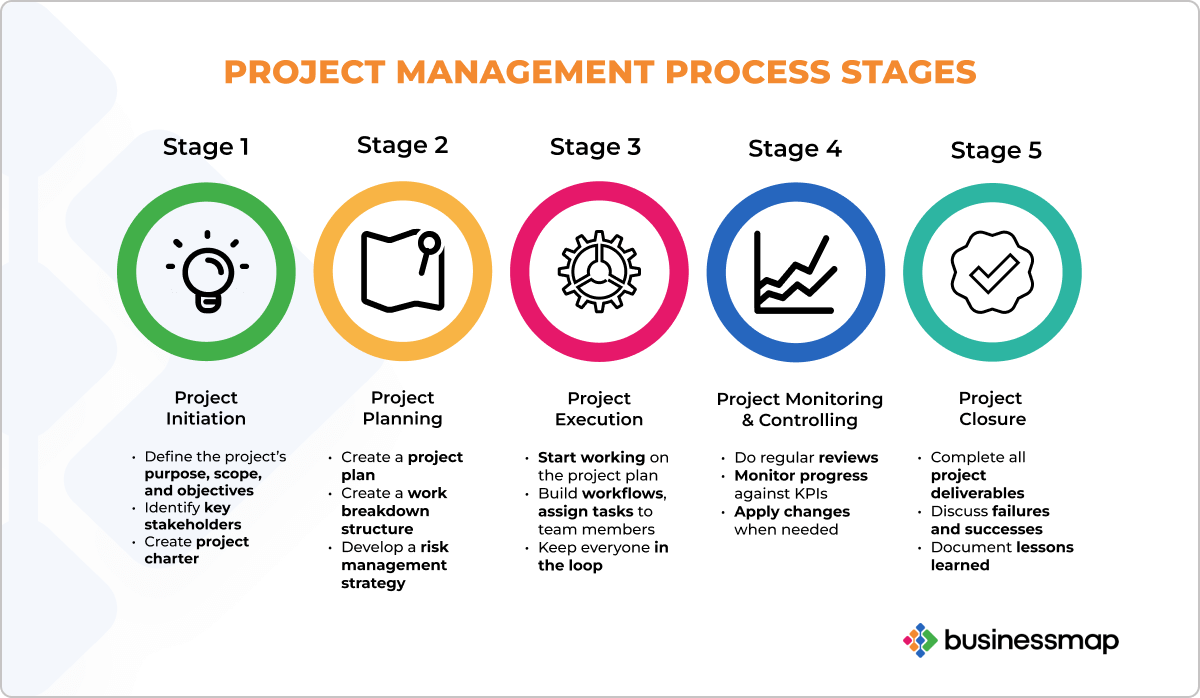
\includegraphics[width=130mm, keepaspectratio]{figures/project_management_process_stages.png}
    \caption{Projektmenedzsment folyamatok fázisai}
    \label{fig:project_management_process_stages}
\end{figure}
%----------------------------------------------------------------------------
